\documentclass[11pt]{article}
\usepackage[margin=2.5cm]{geometry}
\usepackage{booktabs}
\usepackage[hidelinks]{hyperref}
\usepackage{times}
\usepackage{float}
\usepackage{tikz}
\usetikzlibrary{positioning, arrows.meta, calc}
\tikzset{
  nblue/.style={circle, draw=blue!70!black, fill=blue!40, minimum size=5mm, inner sep=0, font=\scriptsize},
  norange/.style={circle, draw=orange!80!black, fill=orange!50, minimum size=5mm, inner sep=0, font=\scriptsize},
  ngreen/.style={circle, draw=green!50!black, fill=green!40, minimum size=5mm, inner sep=0, font=\scriptsize},
  ngray/.style={circle, draw=gray, fill=gray!20, minimum size=5mm, inner sep=0, font=\scriptsize},
  nboth/.style={circle, draw=black, left color=blue!40, right color=orange!50, minimum size=5mm, inner sep=0},
  hub/.style={rectangle, rounded corners=2pt, draw=black, thick, fill=yellow!40, minimum size=6mm, inner sep=1pt, font=\scriptsize\bfseries},
  gedge/.style={gray!70, thick},
  inedge/.style={green!50!black, very thick},
  outedge/.style={red!70!black, very thick, dashed},
  cedge/.style={red!70!black, thick, dashed},
  thinc/.style={red!70!black, densely dotted, thin},
  hedge/.style={black!60, thin},
  hhedge/.style={purple!80!black, very thick},
  box/.style={rectangle, rounded corners=2pt, draw=black, fill=white, minimum height=7mm, inner sep=3pt, font=\footnotesize, align=center},
  newbox/.style={box, fill=yellow!40, thick},
  arr/.style={-{Stealth[length=2mm]}, thick},
  ftitle/.style={font=\small\bfseries},
  fnote/.style={font=\footnotesize, align=center}}

\title{Runs 4--9: Looking for the Gap to GLASS}
\author{}
\date{October 28, 2026}

\begin{document}
\maketitle

Each section answers four questions: why we ran it, what we changed, what came out, and what we
learned. Numbers are test micro-F1 ($\times 100$), mean of 10 seeds. In the figures, yellow marks
what is new in that run.

% ---------------------------------------------------------------- Run 4
\section*{Run 4: normalizing the clique, and the hub graph}
\begin{itemize}
  \item \textbf{Why:} the advisor said the clique (an edge between every two nodes of a subgraph) pulls all its nodes to one vector, which is close to just averaging them.
  \item \textbf{What we changed:} (1) clique messages divided by $\sqrt{d_i d_j}$, as in GCN, where $d$ is a node's number of clique neighbors; (2) the same, with each clique edge also weighted by 1/(subgraph size); (3) a hub graph: one extra node per subgraph, and links between extra nodes of subgraphs that share nodes or edges (Figure~\ref{fig:run4}).
  \item \textbf{Result:} (1) and (2) moved every dataset by less than one std. The hub graph gave our best cut\_ratio at the time (81.6), but no gain elsewhere. Error did not grow with subgraph size.
  \item \textbf{Learned:} how the clique is weighted is not what holds us back.
\end{itemize}

\begin{figure}[H]
\centering
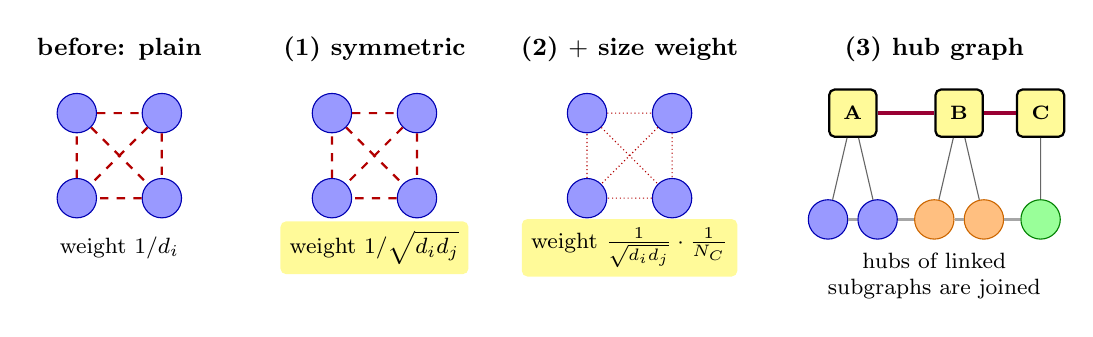
\begin{tikzpicture}[scale=0.9]
  \begin{scope}
    \node[ftitle] at (0.6,2.7) {before: plain};
    \node[nblue] (a) at (0,1.8) {}; \node[nblue] (b) at (1.2,1.8) {};
    \node[nblue] (c) at (1.2,0.6) {}; \node[nblue] (d) at (0,0.6) {};
    \draw[cedge] (a)--(b) (b)--(c) (c)--(d) (d)--(a) (a)--(c) (b)--(d);
    \node[fnote] at (0.6,-0.1) {weight $1/d_i$};
  \end{scope}
  \begin{scope}[xshift=3.6cm]
    \node[ftitle] at (0.6,2.7) {(1) symmetric};
    \node[nblue] (a) at (0,1.8) {}; \node[nblue] (b) at (1.2,1.8) {};
    \node[nblue] (c) at (1.2,0.6) {}; \node[nblue] (d) at (0,0.6) {};
    \draw[cedge] (a)--(b) (b)--(c) (c)--(d) (d)--(a) (a)--(c) (b)--(d);
    \node[fnote, fill=yellow!40, rounded corners=2pt] at (0.6,-0.1) {weight $1/\sqrt{d_i d_j}$};
  \end{scope}
  \begin{scope}[xshift=7.2cm]
    \node[ftitle] at (0.6,2.7) {(2) $+$ size weight};
    \node[nblue] (a) at (0,1.8) {}; \node[nblue] (b) at (1.2,1.8) {};
    \node[nblue] (c) at (1.2,0.6) {}; \node[nblue] (d) at (0,0.6) {};
    \draw[thinc] (a)--(b) (b)--(c) (c)--(d) (d)--(a) (a)--(c) (b)--(d);
    \node[fnote, fill=yellow!40, rounded corners=2pt] at (0.6,-0.1) {weight $\frac{1}{\sqrt{d_i d_j}}\cdot\frac{1}{N_C}$};
  \end{scope}
  \begin{scope}[xshift=10.6cm]
    \node[ftitle] at (1.5,2.7) {(3) hub graph};
    \node[nblue] (a1) at (0,0.3) {}; \node[nblue] (a2) at (0.7,0.3) {};
    \node[norange] (b1) at (1.5,0.3) {}; \node[norange] (b2) at (2.2,0.3) {};
    \node[ngreen] (c1) at (3.0,0.3) {};
    \draw[gedge] (a1)--(a2) (a2)--(b1) (b1)--(b2) (b2)--(c1);
    \node[hub] (HA) at (0.35,1.8) {A}; \node[hub] (HB) at (1.85,1.8) {B}; \node[hub] (HC) at (3.0,1.8) {C};
    \draw[hedge] (HA)--(a1) (HA)--(a2) (HB)--(b1) (HB)--(b2) (HC)--(c1);
    \draw[hhedge] (HA)--(HB) (HB)--(HC);
    \node[fnote] at (1.5,-0.5) {hubs of linked\\ subgraphs are joined};
  \end{scope}
\end{tikzpicture}
\caption{Run 4. Red dashed: clique edges. (1)--(2) change only how much each clique message
counts; thinner means it counts less. (3) adds one hub per subgraph (yellow) and purple links
between hubs of subgraphs that share nodes or are joined by graph edges.}
\label{fig:run4}
\end{figure}

% ---------------------------------------------------------------- GLASS check
\section*{Check: the GLASS paper}
\begin{itemize}
  \item \textbf{Why:} to see what GLASS does that we do not.
  \item \textbf{What we found:} GLASS also reports a plain GNN, with no marks telling the model which nodes are in the subgraph (Figure~\ref{fig:glass}). It gets 59.7 on hpo\_metab and 66.8 on hpo\_neuro, about 4 points above our best at the time.
  \item \textbf{Learned:} a simple model beats us on the real datasets, so the gap is not about how we mark subgraphs. The question became: what is different in our setup?
\end{itemize}

\begin{figure}[H]
\centering
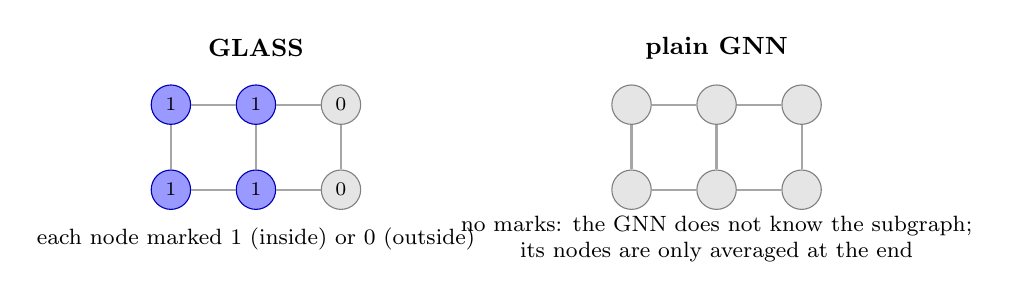
\begin{tikzpicture}[scale=0.9]
  \begin{scope}
    \node[ftitle] at (1.2,2.6) {GLASS};
    \node[nblue] (a) at (0,1.8) {1}; \node[nblue] (b) at (1.2,1.8) {1};
    \node[nblue] (c) at (1.2,0.6) {1}; \node[nblue] (d) at (0,0.6) {1};
    \node[ngray] (e) at (2.4,1.8) {0}; \node[ngray] (f) at (2.4,0.6) {0};
    \draw[gedge] (a)--(b) (b)--(c) (c)--(d) (d)--(a) (b)--(e) (c)--(f) (e)--(f);
    \node[fnote] at (1.2,-0.1) {each node marked 1 (inside) or 0 (outside)};
  \end{scope}
  \begin{scope}[xshift=6.5cm]
    \node[ftitle] at (1.2,2.6) {plain GNN};
    \node[ngray] (a) at (0,1.8) {}; \node[ngray] (b) at (1.2,1.8) {};
    \node[ngray] (c) at (1.2,0.6) {}; \node[ngray] (d) at (0,0.6) {};
    \node[ngray] (e) at (2.4,1.8) {}; \node[ngray] (f) at (2.4,0.6) {};
    \draw[gedge] (a)--(b) (b)--(c) (c)--(d) (d)--(a) (b)--(e) (c)--(f) (e)--(f);
    \node[fnote] at (1.2,-0.1) {no marks: the GNN does not know the subgraph;\\ its nodes are only averaged at the end};
  \end{scope}
\end{tikzpicture}
\caption{GLASS and its plain GNN, on a subgraph of four nodes. The plain GNN is the simplest
possible model, and it still beats us on hpo.}
\label{fig:glass}
\end{figure}

% ---------------------------------------------------------------- Run 5
\section*{Run 5: node copies and split edges}
\begin{itemize}
  \item \textbf{Why:} on density and hpo, many nodes are in more than one subgraph, so one node vector has to serve several subgraphs.
  \item \textbf{What we changed:} (1) copies: each node gets a separate copy for each subgraph it is in; (2) split edges: graph edges inside a subgraph and edges leaving it get separate weights (Figure~\ref{fig:run5}); (3) input vectors started from SubGNN's pretrained ones.
  \item \textbf{Result:} copies lifted density from 78.8 to 92.4, but lowered cut\_ratio and component. Split edges gave our best hpo (metab 59.7, neuro 64.1) but broke density (34.4). SubGNN's vectors gave nothing.
  \item \textbf{Learned:} each idea fixes some datasets and breaks others.
\end{itemize}

\begin{figure}[H]
\centering
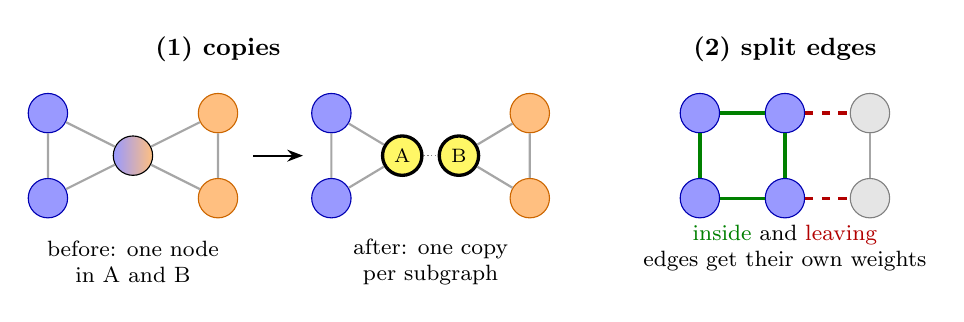
\begin{tikzpicture}[scale=0.9]
  \begin{scope}
    \node[ftitle] at (2.4,2.7) {(1) copies};
    \node[nblue] (a1) at (0,1.8) {}; \node[nblue] (a2) at (0,0.6) {};
    \node[nboth] (s) at (1.2,1.2) {};
    \node[norange] (b1) at (2.4,1.8) {}; \node[norange] (b2) at (2.4,0.6) {};
    \draw[gedge] (a1)--(a2) (a1)--(s) (a2)--(s) (s)--(b1) (s)--(b2) (b1)--(b2);
    \node[fnote] at (1.2,-0.3) {before: one node\\ in A and B};
    \draw[arr] (2.9,1.2)--(3.6,1.2);
    \node[nblue] (A1) at (4.0,1.8) {}; \node[nblue] (A2) at (4.0,0.6) {};
    \node[nblue, draw=black, very thick, fill=yellow!60] (sA) at (5.0,1.2) {A};
    \node[norange, draw=black, very thick, fill=yellow!60] (sB) at (5.8,1.2) {B};
    \node[norange] (B1) at (6.8,1.8) {}; \node[norange] (B2) at (6.8,0.6) {};
    \draw[gedge] (A1)--(A2) (A1)--(sA) (A2)--(sA) (sB)--(B1) (sB)--(B2) (B1)--(B2);
    \draw[gray, thin, densely dotted] (sA)--(sB);
    \node[fnote] at (5.4,-0.3) {after: one copy\\ per subgraph};
  \end{scope}
  \begin{scope}[xshift=9.2cm]
    \node[ftitle] at (1.2,2.7) {(2) split edges};
    \node[nblue] (a) at (0,1.8) {}; \node[nblue] (b) at (1.2,1.8) {};
    \node[nblue] (c) at (1.2,0.6) {}; \node[nblue] (d) at (0,0.6) {};
    \node[ngray] (e) at (2.4,1.8) {}; \node[ngray] (f) at (2.4,0.6) {};
    \draw[inedge] (a)--(b) (b)--(c) (c)--(d) (d)--(a);
    \draw[outedge] (b)--(e) (c)--(f);
    \draw[gedge] (e)--(f);
    \node[fnote] at (1.2,-0.1) {\textcolor{green!50!black}{inside} and \textcolor{red!70!black}{leaving}\\ edges get their own weights};
  \end{scope}
\end{tikzpicture}
\caption{Run 5. (1) The half-blue, half-orange node is in subgraphs A and B; it is replaced by
two copies (yellow), each linked only to its own subgraph. (2) Graph edges are split into two
types by whether they stay inside a subgraph.}
\label{fig:run5}
\end{figure}

% ---------------------------------------------------------------- Run 6
\section*{Run 6: copies plus edge counts}
\begin{itemize}
  \item \textbf{Why:} in run 5, copies fixed density but lowered cut\_ratio (66.0) and component (67.6). Cut\_ratio is about how many edges leave the subgraph, and a copy has no direct way to see that. So we tried to hand it this number.
  \item \textbf{What we changed:} we kept run 5's copies model, and gave each copy two numbers as extra input: how many of its graph edges stay inside its subgraph, and how many leave it (Figure~\ref{fig:run6}).
  \item \textbf{Result:} component recovered (67.6 $\to$ 98.0) and density rose to 94.4, our best and above GLASS (93.0). Cut\_ratio did not move (66.0 $\to$ 66.8). The real datasets stayed below our best.
  \item \textbf{Learned:} the model was given the exact numbers cut\_ratio depends on, and still did not use them. This made us suspect the training, which run 7 checks.
\end{itemize}

\begin{figure}[H]
\centering
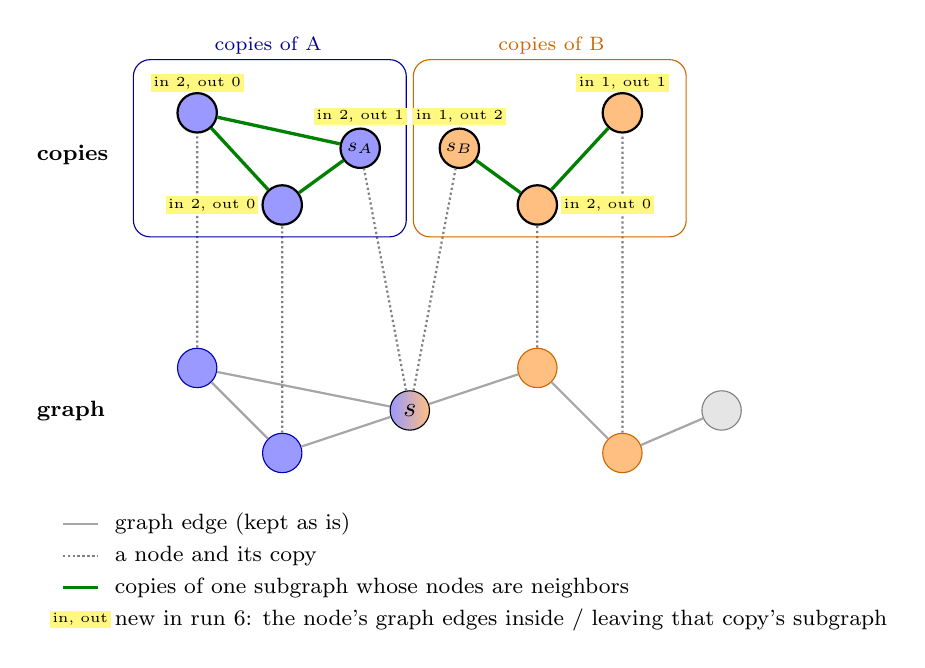
\begin{tikzpicture}[scale=0.9]
  % ---- original graph (kept as is)
  \node[font=\footnotesize\bfseries, anchor=west] at (-3.4,0) {graph};
  \node[nblue] (a1) at (-1.0,0.6) {}; \node[nblue] (a2) at (0.2,-0.6) {};
  \node[nboth] (s) at (2,0) {$s$};
  \node[norange] (b1) at (3.8,0.6) {}; \node[norange] (b2) at (5.0,-0.6) {};
  \node[ngray] (g) at (6.4,0) {};
  \draw[gedge] (a1)--(a2) (a1)--(s) (a2)--(s) (s)--(b1) (b1)--(b2) (b2)--(g);
  % ---- copies: one per (node, subgraph)
  \node[font=\footnotesize\bfseries, anchor=west] at (-3.4,3.6) {copies};
  \node[nblue, draw=black, thick] (ca1) at (-1.0,4.2) {}; \node[nblue, draw=black, thick] (ca2) at (0.2,2.9) {};
  \node[nblue, draw=black, thick] (csA) at (1.3,3.7) {$s_A$};
  \node[norange, draw=black, thick] (csB) at (2.7,3.7) {$s_B$};
  \node[norange, draw=black, thick] (cb1) at (3.8,2.9) {}; \node[norange, draw=black, thick] (cb2) at (5.0,4.2) {};
  \draw[inedge] (ca1)--(ca2) (ca1)--(csA) (ca2)--(csA) (csB)--(cb1) (cb1)--(cb2);
  \draw[gray, densely dotted, thick] (a1)--(ca1) (a2)--(ca2) (s)--(csA) (s)--(csB) (b1)--(cb1) (b2)--(cb2);
  \draw[blue!60!black, rounded corners=6pt, thin] (-1.9,2.45) rectangle (1.95,4.95);
  \node[font=\scriptsize, blue!60!black] at (0.0,5.15) {copies of A};
  \draw[orange!80!black, rounded corners=6pt, thin] (2.05,2.45) rectangle (5.9,4.95);
  \node[font=\scriptsize, orange!80!black] at (4.0,5.15) {copies of B};
  % counts (yellow)
  \node[font=\tiny, fill=yellow!50, inner sep=1pt] at (-1.0,4.62) {in 2, out 0};
  \node[font=\tiny, fill=yellow!50, inner sep=1pt, anchor=east] at ([xshift=-1pt]ca2.west) {in 2, out 0};
  \node[font=\tiny, fill=yellow!50, inner sep=1pt] at (1.3,4.15) {in 2, out 1};
  \node[font=\tiny, fill=yellow!50, inner sep=1pt] at (2.7,4.15) {in 1, out 2};
  \node[font=\tiny, fill=yellow!50, inner sep=1pt, anchor=west] at ([xshift=1pt]cb1.east) {in 2, out 0};
  \node[font=\tiny, fill=yellow!50, inner sep=1pt] at (5.0,4.62) {in 1, out 1};  % ---- legend
  \begin{scope}[yshift=-1.6cm, xshift=-2.9cm]
    \draw[gedge] (0,0)--(0.5,0); \node[fnote, anchor=west] at (0.6,0) {graph edge (kept as is)};
    \draw[gray, densely dotted, thick] (0,-0.45)--(0.5,-0.45); \node[fnote, anchor=west] at (0.6,-0.45) {a node and its copy};
    \draw[inedge] (0,-0.9)--(0.5,-0.9); \node[fnote, anchor=west] at (0.6,-0.9) {copies of one subgraph whose nodes are neighbors};
    \node[font=\tiny, fill=yellow!50, inner sep=1pt] at (0.25,-1.35) {in, out};
    \node[fnote, anchor=west] at (0.6,-1.35) {new in run 6: the node's graph edges inside / leaving that copy's subgraph};
  \end{scope}\end{tikzpicture}
\caption{Run 6, the whole graph. Node $s$ is in subgraphs A (blue) and B (orange). Every
(node, subgraph) pair gets its own copy, so $s$ gets two: $s_A$ and $s_B$. The original graph
stays, each node is linked to its copies, and copies of one subgraph are linked when their nodes
are neighbors in the graph. New in run 6 are the yellow counts. They are counted on the
original graph from the copy's subgraph's side, so the same node $s$ gets (2, 1) for A and
(1, 2) for B.}\label{fig:run6}
\end{figure}

% ---------------------------------------------------------------- Run 7
\section*{Run 7: is it the model or the training?}
\begin{itemize}
  \item \textbf{Why:} to find out whether our model cannot express the answer, or our training cannot find it.
  \item \textbf{What we changed:} (1) the subgraph's exact counts (size, inside edges, outside edges) fed straight to the final classifier; (2) GLASS's plain GNN rebuilt in our code (Figure~\ref{fig:run7}).
  \item \textbf{Result:} (1) cut\_ratio 68.4, and the model fit only 85\% of its own training subgraphs. (2) ppi\_bp 62.8 (as good as GLASS), but hpo\_metab 46.6 (13 below GLASS).
  \item \textbf{Learned:} the model has what it needs but does not learn it, so the problem is our training.
\end{itemize}

\begin{figure}[H]
\centering
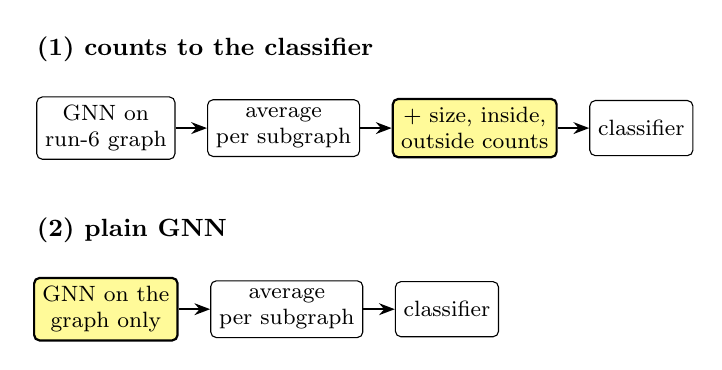
\begin{tikzpicture}[node distance=4mm]
  \node[ftitle, anchor=west] at (-1.0,1.0) {(1) counts to the classifier};
  \node[box] (g) at (0,0) {GNN on\\ run-6 graph};
  \node[box, right=of g] (p) {average\\ per subgraph};
  \node[newbox, right=of p] (k) {$+$ size, inside,\\ outside counts};
  \node[box, right=of k] (cl) {classifier};
  \draw[arr] (g)--(p); \draw[arr] (p)--(k); \draw[arr] (k)--(cl);
  \node[ftitle, anchor=west] at (-1.0,-1.3) {(2) plain GNN};
  \node[newbox] (g2) at (0,-2.3) {GNN on the\\ graph only};
  \node[box, right=of g2] (p2) {average\\ per subgraph};
  \node[box, right=of p2] (cl2) {classifier};
  \draw[arr] (g2)--(p2); \draw[arr] (p2)--(cl2);
\end{tikzpicture}
\caption{Run 7. (1) The classifier gets the exact counts that define density and cut\_ratio, so
it only has to learn to read them. (2) No clique, no copies, no hubs: the simplest model, as in
GLASS's plain GNN.}
\label{fig:run7}
\end{figure}

% ---------------------------------------------------------------- Run 8
\section*{Run 8: training like GLASS}
\begin{itemize}
  \item \textbf{Why:} GLASS normalizes after each GNN layer and trains on small batches; we did neither.
  \item \textbf{What we changed:} added both to the models of run 7 (Figure~\ref{fig:run8}).
  \item \textbf{Result:} cut\_ratio 76.0 (now fits 98\% of training), coreness 85.2 (above GLASS). The plain GNN on hpo\_metab did not move (46.5).
  \item \textbf{Learned:} normalization fixes part of the synthetic gap, but not hpo\_metab.
\end{itemize}

\begin{figure}[H]
\centering
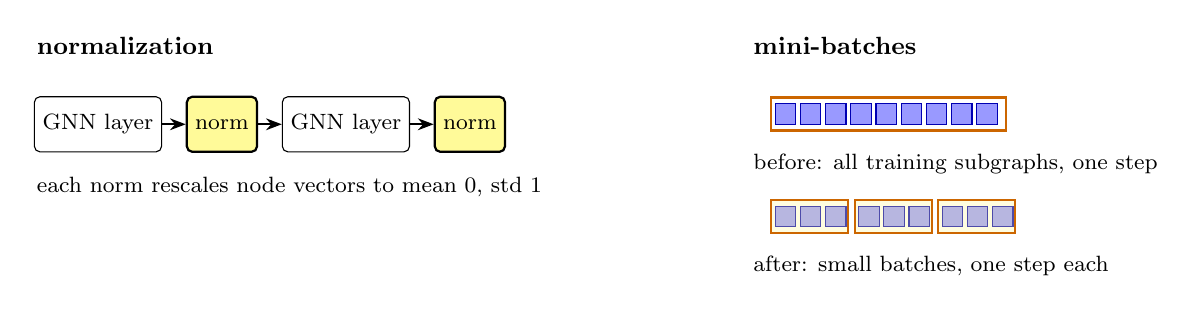
\begin{tikzpicture}[node distance=3mm]
  \node[ftitle, anchor=west] at (-0.9,1.0) {normalization};
  \node[box] (l1) at (0,0) {GNN layer};
  \node[newbox, right=of l1] (n1) {norm};
  \node[box, right=of n1] (l2) {GNN layer};
  \node[newbox, right=of l2] (n2) {norm};
  \draw[arr] (l1)--(n1); \draw[arr] (n1)--(l2); \draw[arr] (l2)--(n2);
  \node[fnote, anchor=west] at (-0.9,-0.8) {each norm rescales node vectors to mean 0, std 1};
  \begin{scope}[xshift=8.6cm]
    \node[ftitle, anchor=west] at (-0.4,1.0) {mini-batches};
    \foreach \i in {0,...,8} { \fill[blue!40, draw=blue!70!black] ({\i*0.32},0) rectangle ++(0.26,0.26); }
    \draw[thick, orange!80!black] (-0.05,-0.08) rectangle (2.93,0.34);
    \node[fnote, anchor=west] at (-0.4,-0.5) {before: all training subgraphs, one step};
    \foreach \i in {0,...,8} { \fill[blue!40, draw=blue!70!black] ({\i*0.32+0.1*int(\i/3)},-1.3) rectangle ++(0.26,0.26); }
    \foreach \j in {0,1,2} { \draw[thick, orange!80!black, fill=yellow!40, fill opacity=0.3] ({\j*1.06-0.05},-1.38) rectangle ++(0.98,0.42); }
    \node[fnote, anchor=west] at (-0.4,-1.8) {after: small batches, one step each};
  \end{scope}
\end{tikzpicture}
\caption{Run 8. Two training changes copied from GLASS; the model itself is the same as in run 7.}
\label{fig:run8}
\end{figure}

% ---------------------------------------------------------------- Run 9
\section*{Run 9: GLASS's own input vectors}
\begin{itemize}
  \item \textbf{Why:} the input was the last difference we could see.
  \item \textbf{What we changed:} started from GLASS's own pretrained node vectors (Figure~\ref{fig:run9}).
  \item \textbf{Result:} plain GNN: hpo\_metab 50.0 (still 10 below), hpo\_neuro 66.0 (equal to GLASS's plain GNN). Split edges: ppi\_bp 64.0, our best ever, above GLASS.
  \item \textbf{Learned:} same input and nearly the same model, and hpo\_metab is still far behind. We do not know why.
\end{itemize}

\begin{figure}[H]
\centering
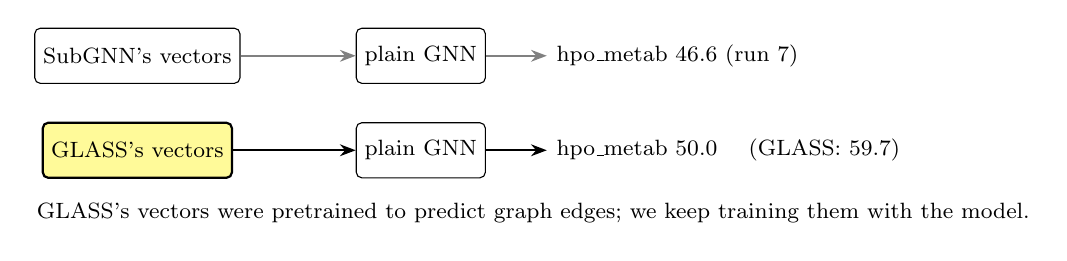
\begin{tikzpicture}[node distance=4mm]
  \node[box] (s) at (0,0) {SubGNN's vectors};
  \node[newbox] (gl) at (0,-1.2) {GLASS's vectors};
  \node[box] (g1) at (3.6,0) {plain GNN};
  \node[box] (g2) at (3.6,-1.2) {plain GNN};
  \draw[arr, gray] (s)--(g1);
  \draw[arr] (gl)--(g2);
  \node[fnote, anchor=west] (o1) at (5.2,0) {hpo\_metab 46.6 (run 7)};
  \node[fnote, anchor=west] (o2) at (5.2,-1.2) {hpo\_metab 50.0 \quad (GLASS: 59.7)};
  \draw[arr, gray] (g1)--(o1); \draw[arr] (g2)--(o2);
  \node[fnote, anchor=west] at (-1.4,-2.0) {GLASS's vectors were pretrained to predict graph edges; we keep training them with the model.};
\end{tikzpicture}
\caption{Run 9. Only the starting node vectors change. Gray: the input used before.}
\label{fig:run9}
\end{figure}

% ---------------------------------------------------------------- Now
\section*{Now: running GLASS's own code}
\begin{itemize}
  \item \textbf{Why:} to see if GLASS's published numbers can be reached on our server at all.
  \item \textbf{What we are doing:} running the authors' code with their settings on all 8 datasets, for both full GLASS and its plain GNN (Figure~\ref{fig:now}). (GPEN has no public code.)
  \item \textbf{What it will tell us:} if their plain GNN gets about 60 on hpo\_metab, we compare their code with ours step by step. If not, the published number is hard to reach.
  \item \textbf{Already found in their code:} when several epochs tie on validation, it reports the best test score among them; and their ``$\pm$'' is std$/\sqrt{10}$, smaller than the std we report.
\end{itemize}

\begin{figure}[H]
\centering
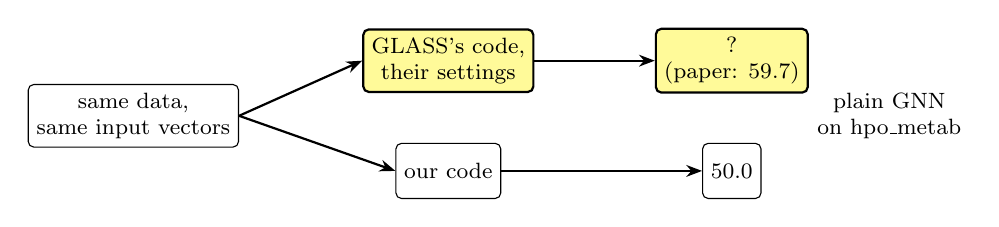
\begin{tikzpicture}[node distance=5mm]
  \node[box] (d) at (0,0) {same data,\\ same input vectors};
  \node[newbox] (gc) at (4.0,0.7) {GLASS's code,\\ their settings};
  \node[box] (oc) at (4.0,-0.7) {our code};
  \node[newbox] (gr) at (7.6,0.7) {? \\ (paper: 59.7)};
  \node[box] (or) at (7.6,-0.7) {50.0};
  \draw[arr] (d.east)--(gc.west); \draw[arr] (d.east)--(oc.west);
  \draw[arr] (gc)--(gr); \draw[arr] (oc)--(or);
  \node[fnote] at (9.6,0) {plain GNN\\ on hpo\_metab};
\end{tikzpicture}
\caption{The run going now. If the top line reaches about 60, the gap is in our code and we can
find it by comparing the two step by step.}
\label{fig:now}
\end{figure}

% ---------------------------------------------------------------- Summary
\begin{table}[H]
\centering
\small
\begin{tabular}{lclc}
\toprule
dataset & our best & from & GLASS \\
\midrule
ppi\_bp    & 64.0 & run 9, split edges + GLASS vectors & 61.9 \\
hpo\_metab & 59.7 & run 5, split edges                 & 61.4 \\
hpo\_neuro & 66.0 & run 9, plain GNN + GLASS vectors   & 68.5 \\
density    & 94.4 & run 6, copies + counts             & 93.0 \\
cut\_ratio & 81.6 & run 4, hub graph                   & 93.5 \\
coreness   & 89.1 & run 3, transformer readout         & 84.0 \\
component  & 100.0 & run 7, counts to classifier       & 100.0 \\
\bottomrule
\end{tabular}
\caption{Test micro-F1 ($\times 100$), mean over 10 seeds. ``Our best'' is the best of runs
2--9 on each dataset, from different models. GLASS numbers are from the GLASS paper.}
\end{table}

\end{document}
